
%(BEGIN_QUESTION)
% Copyright 2008, Tony R. Kuphaldt, released under the Creative Commons Attribution License (v 1.0)
% This means you may do almost anything with this work of mine, so long as you give me proper credit

This liquid level sensor circuit uses a plastic-coated metal rod as one ``plate'' of a capacitor, and the metal vessel as the other ``plate'' of the capacitor:

$$\includegraphics[width=15.5cm]{i02918x01.eps}$$

Sketch an equivalent circuit showing the level sensing probe as an ideal circuit element, and then determine the following if the liquid level in the vessel happens to increase:

\begin{itemize}
\item{} Probe capacitance: ({\it increase}, {\it decrease}, or {\it remain the same})
\vskip 10pt 
\item{} Capacitive reactance: ({\it increase}, {\it decrease}, or {\it remain the same})
\vskip 10pt 
\item{} AC voltage between point {\bf A} and ground: ({\it increase}, {\it decrease}, or {\it remain the same})
\end{itemize}

\vfil 

\underbar{file i02918}
\eject
%(END_QUESTION)





%(BEGIN_ANSWER)

This is a graded question -- no answers or hints given!

%(END_ANSWER)





%(BEGIN_NOTES)

$$\includegraphics[width=15.5cm]{i02918x02.eps}$$

As level increases, so does the effective surface area of the vessel (acting as a capacitor plate).  This increases capacitance ($C$), decreasing capacitive reactance ($X_C$), and increasing circuit current ($I$).  An increase in current drops more AC voltage across the resistor, leaving less voltage between point {\bf A} and ground. 

\begin{itemize}
\item{} Probe capacitance: will {\bf increase}
\vskip 10pt 
\item{} Capacitive reactance: will {\bf decrease}
\vskip 10pt 
\item{} AC voltage between point {\bf A} and ground will {\bf decrease}
\end{itemize}

A vitally important general principle of electric circuits is that voltage is always measured between {\it two} points, not at one point.  Whenever you need to determine a particular voltage, you must identify which {\it two} points in the circuit that voltage lies between.  In the case of ``A'' and ground, the voltage in question spans the dielectric sheath around the probe, not across the resistor.

%INDEX% Electronics review: qualitative analysis of simple AC circuit

%(END_NOTES)


